% 45-45-90 边比 1 : 1 : √2
\documentclass[tikz,border=4pt]{standalone}
\usepackage{ctex}
\usepackage{amsmath}
\usetikzlibrary{decorations.markings}
\begin{document}
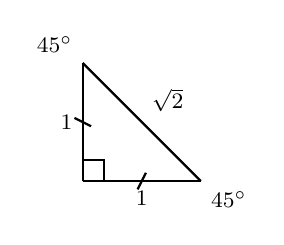
\begin{tikzpicture}[scale=1.5, thick,
  tick/.style={postaction={decorate, decoration={markings,
    mark=at position 0.5 with {\draw (-1.5pt,-3pt) -- (1.5pt,3pt);}}}}]
  \coordinate (A) at (0,0);
  \coordinate (B) at (1,0);
  \coordinate (C) at (0,1);
  \draw[tick] (A) -- (B);
  \draw[tick] (A) -- (C);
  \draw (B) -- (C);
  \draw (0.18,0) -- (0.18,0.18) -- (0,0.18);
  \node[below] at (0.5, 0)   {\footnotesize $1$};
  \node[left]  at (0, 0.5)   {\footnotesize $1$};
  \node[above right] at (0.5, 0.5) {\footnotesize $\sqrt{2}$};
  \node[below right] at (B) {\footnotesize $45^\circ$};
  \node[above left]  at (C) {\footnotesize $45^\circ$};
\end{tikzpicture}
\end{document}
